% owner: jeff
\chapter{Kontext und "Uberblick}
\label{cha:kont}

\section{Systemumgebung}
Das System wird in einem bereits bestehenden Computer-Netzwerk verwendet. Zu
diesem gehören sowohl die einzelnen Computer als Netzwerkknoten, als auch
sämtliche Peripherie zum Verbinden dieser Knoten untereinander. Das System
ist auf Empfangsseite mit älteren Versionen
der MultiCast-Testing-Software kompatibel.

\section{Systemgrenze}
Das System ist klar auf die Anwendungsschicht beschränkt. Es sollen weder auf
Hardware- noch Betriebssystemebene neue Multicasting-Fähigkeiten implementiert, sondern ausschließlich bereits vorhande Implementierungen genutzt und
getestet werden. Interaktion mit anderen Softwarekomponenten auf
Schnittstellenebene ist nich vorgesehen.

\section{Technischer Kontext}
Die folgende Beschreibung konzentriert sich hauptsächlich auf die 
Netzwerktechnologien, mit denen das Tool direkt in Berührung kommt.

\subsection{IP-Multicasting}
Die Kernfunktionalität des Tools ist auf das im IP-Protokoll spezifizierte
Multicasting zurückzuführen.

\begin{figure}
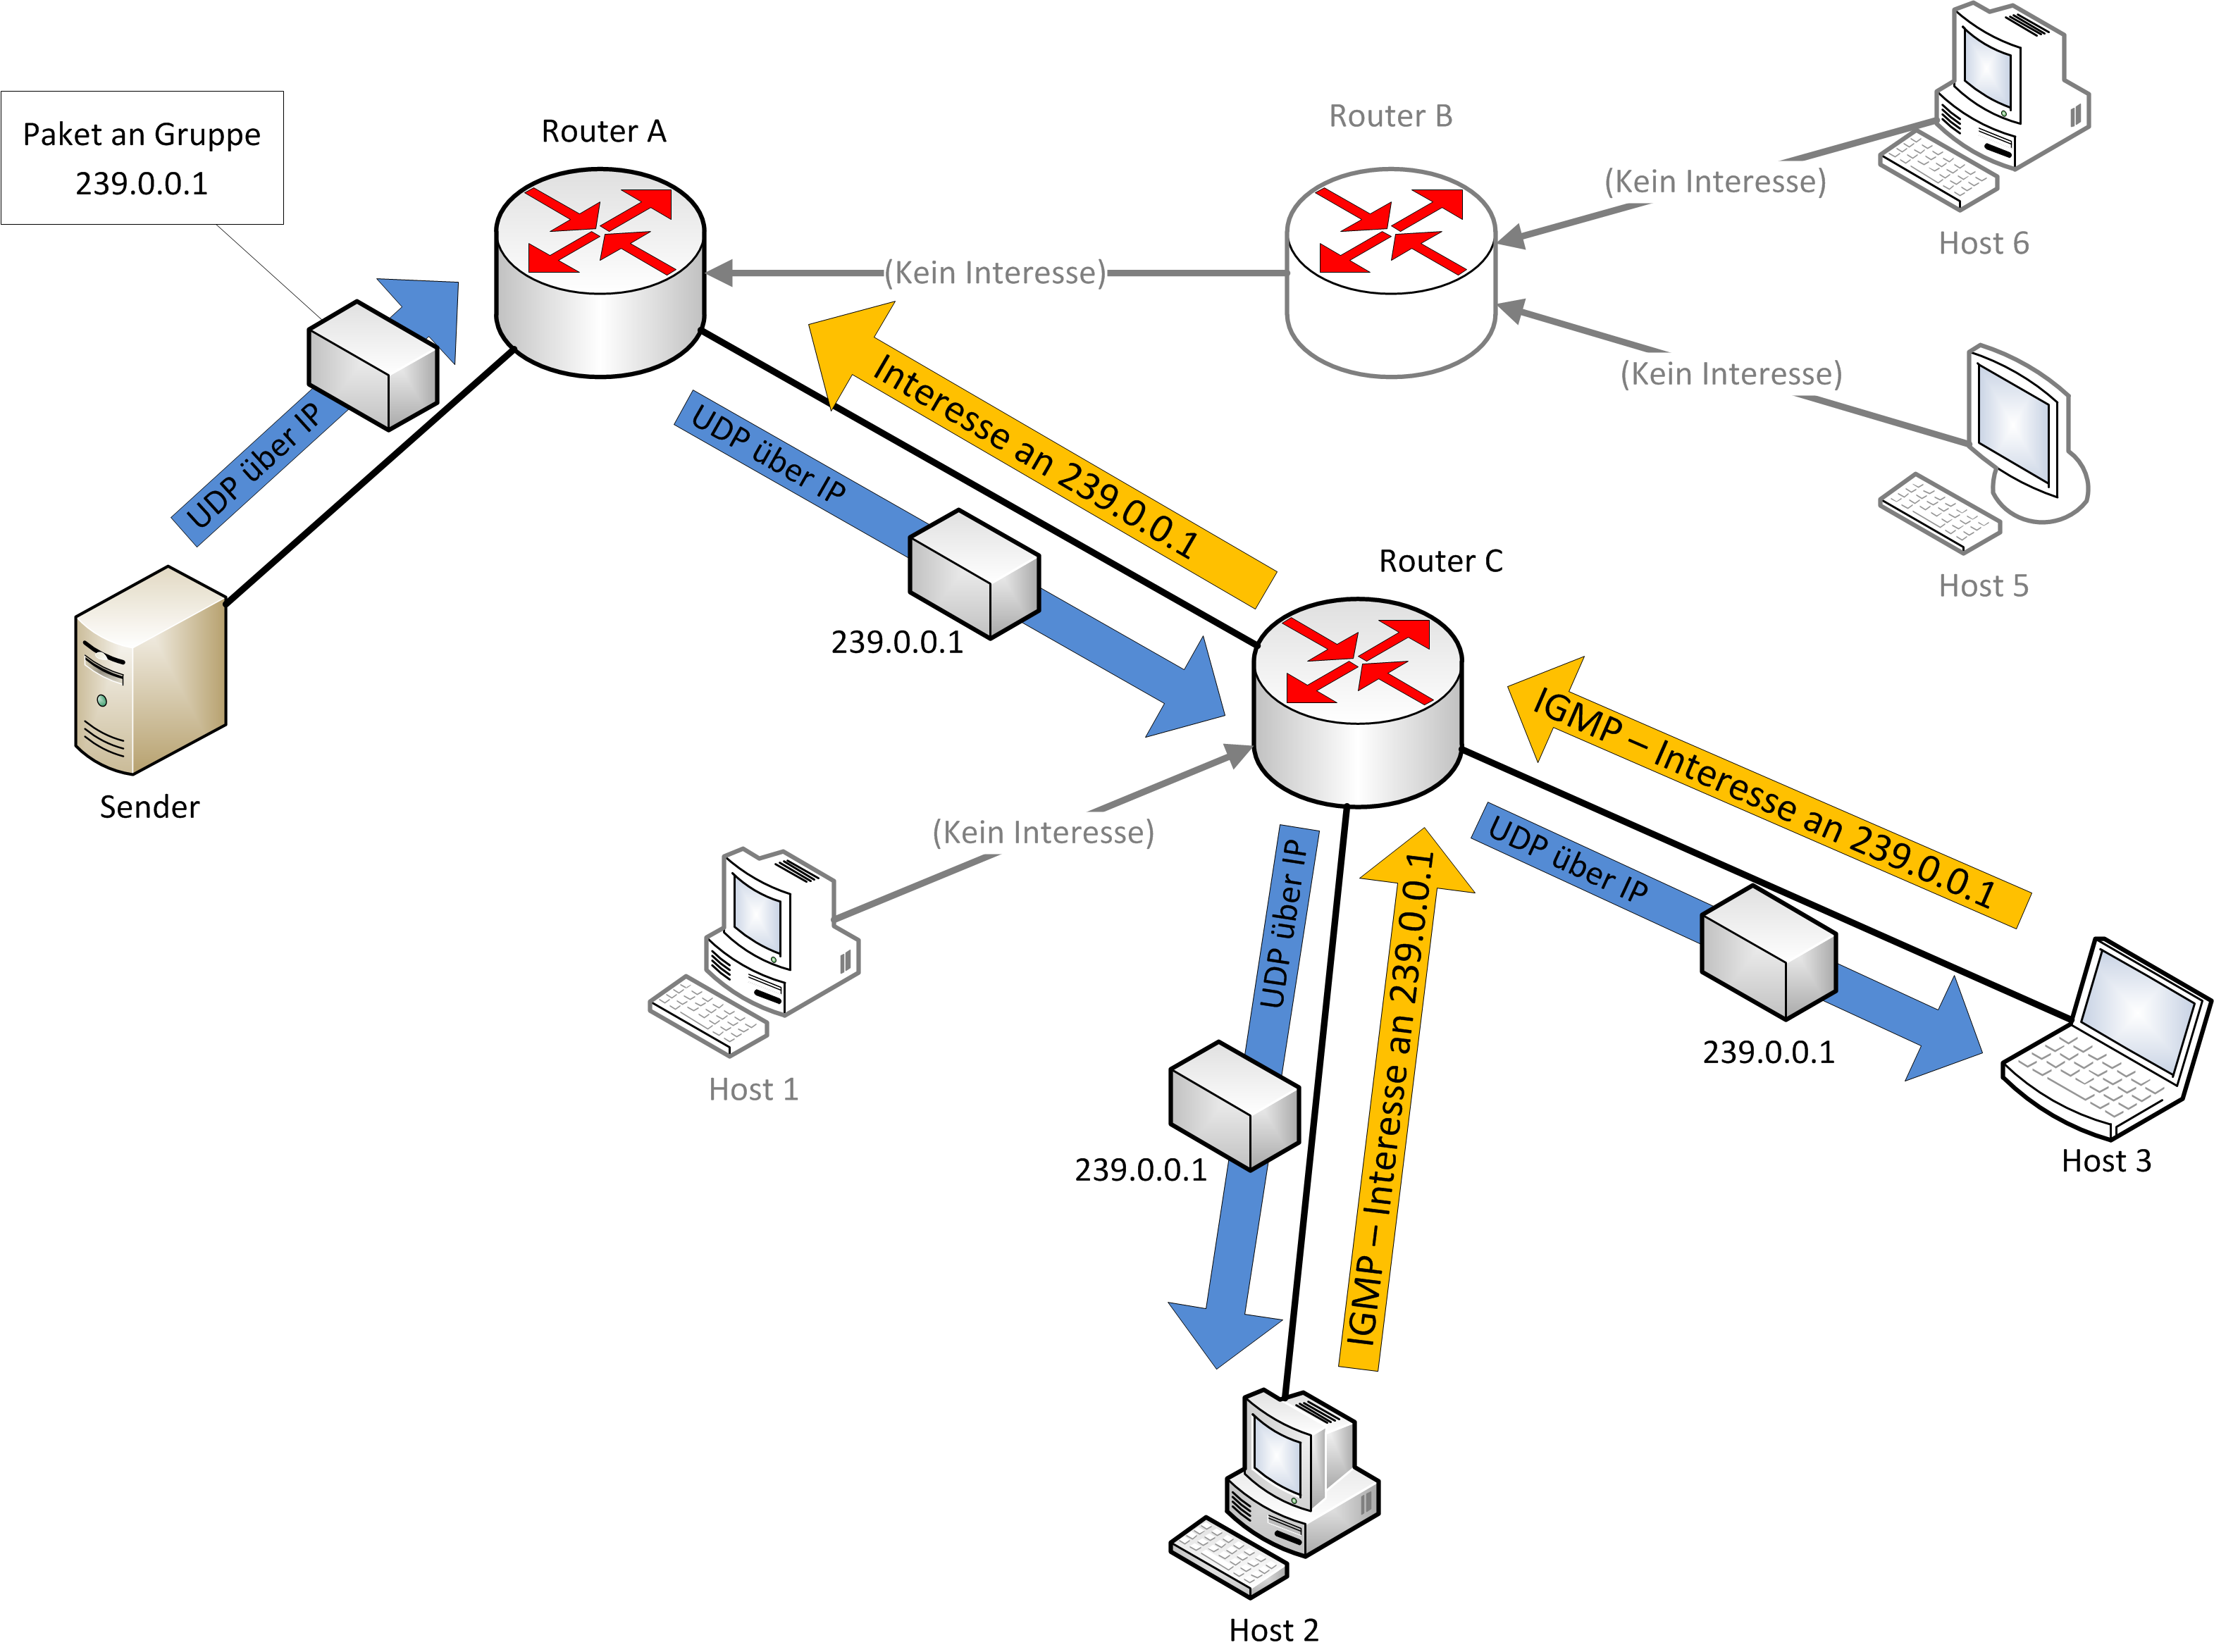
\includegraphics[width=15cm]{images/multicasting.png}
\centering
\caption{Schematische Verteilung eines Multicast-Pakets}
\label{mc_overview}
\end{figure}

\subsubsection{Multicasts senden (Multicast-Adressierung)}
Die Grundlage des Multicastings ist ein bestimmtes
Adressierungsschema auf IP-Ebene (OSI-Layer 3).\\
\\
Das Konzept besteht darin, Pakete nicht direkt an einzelne Hosts, sondern in
eine Multicast-Gruppe zu schicken. Ein Paket wird an eine solche Gruppe adressiert,
indem eine der in RFC3171 spezifizierten Multicast-IP-Adressen als
Empfänger angegeben wird. Der Adressraum für Multicast-Gruppen umfasst die IP-Adressen zwischen
224.0.0.0 und 239.255.255.255. Eine Multicast-Adresse identifiziert genau eine
Multicast-Gruppe. Eine Multicast-Gruppe wird also in diesem Sinne dadurch
"`eröffnet"', dass mindestens ein Host mindestens ein Paket an
ihre Adresse sendet.\\
\\
Für darüberliegende Netzwerkschichten stellt sich diese
Adressierung als transparente IP-Adressierung dar. In der Theorie könnten nun
also auf IP aufsetzende Protokolle auf gewohnte Art und Weise genutzt werden. In
der Praxis ergibt sich allerdings das Problem, dass hinter der Empfängeradresse
eines Pakets nicht der tatsächliche Empfänger, sondern nur die vermittelnde
Multicast-Gruppe steckt. Da eine direkte Zuordnung von Sender und Empfänger so
nicht möglich ist, können Protokolle, die auf eine direkte Verbindung zwischen
zwei Hosts angewiesen sind, nicht ohne weiteres für IP-Multicasting verwendet
werden. Damit scheidet zum Beispiel das weit verbreitete TCP-Protokoll zur
Datenübermittlung aus. Eine Alternative bietet das
UDP-Protokoll, das ohne zuverlässige Verbindungen auskommt.\\
\\
Das Multicast Test Tool realisiert das Multicasten von
UDP-Paketen.

\subsubsection{Multicasts empfangen (IGMP)}
Um IP-Multicasts empfangen zu können, muss ein Host dem Router, an den er
angeschlossen ist, mitteilen, dass er an einer bestimmten Multicastgruppe
interessiert ist. Die gewünschte Gruppe wird wieder über eine
IP-Multicast-Adresse identifiziert. Diese Anmeldung des Hosts für eine
Multicastgruppe wird über das IGMP-Protokoll ausgehandelt. Im Anschluss "`weiß"'
der Router, welcher Host an welchem Anschluss an den Datenpaketen mit einer
bestimmten IP-Gruppen-Adresse im Empfängerfeld interessiert ist.\\
\\
Auch hier fällt
auf, dass der Empfänger keinerlei Wissen über den Sender des Datenstroms
benötigt. Ist er an den Paketen eines bestimmten Hosts interessiert, genügt es
die Adresse zu kennen, \emph{an die} der Host sendet. Es ist sogar die Anmeldung
an einer Gruppe möglich, in die momentan von keinem Host Daten gesendet
werden.\\
\\
In einem Netzwerk mit mehreren Routern, sorgen spezielle
Multicast-Routing-Protokolle dafür, dass die Multicast-Pakete alle
interessierten Hosts auch über mehrere Netzwerkknoten hinweg erreichen.
Dieselben Protokolle sorgen auch dafür, dass solche Pakete wirklich nur die
Router erreichen, deren angeschlossene Hosts oder Netzwerke die jeweilige
Multicast-Gruppe abonniert haben. Beispiele für solche Protokolle sind das
\emph{Distance-Vector Multicast Routing Protocol (DVMRP)} oder das
\emph{Protocol-Independent Multicast (PIM) routing protocol}.

Abbildung \ref{mc_overview} zeigt einen schematischen Überblick über das Senden
und Empfangen eines Multicast-Pakets.

\subsection{Systemkontext}

\begin{figure}[H]
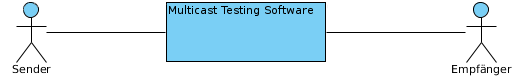
\includegraphics[width=10cm]{images/kontext-usecase.png}
\centering
\caption{Grundsätzlicher Anwendungsfall}
\end{figure}

Das System wird auschließlich in lokalen Netzwerken (LAN) verwendet - eine
Verwendung über das Internet hinweg ist nicht vorgesehen.
Empfangsintervall- und Traversierungszeiten sind in Auflösung von Millisekunden
zu ermitteln.\\
\\
Für die Implementierung wird davon ausgegangen, dass die
beteiligten Netzwerkkomponenten nach RFC1112 Level-2-IP-Multicast-konform sind.
Das bedeutet, dass alle Komponenten (insbesondere alle Router des Netzwerks) das
IGMP-Protokoll implementieren. Sie müssen also sowohl das Senden, als auch das
Abonnieren von Multicast-Datenströmen zulassen, sowie die Datenströme an die
korrekten Empfänger weiterleiten. Eine fehlerhafte Multicasting-Implementierung
der Netzwerkkomponenten wird sich in der Anwendung in Form verlorener Pakete
widerspiegeln.\\
\\
Aus OSI-Layer-Sicht interagiert unsere Anwendung zunächst direkt
(bzw. über die JVM) mit UDP, also Layer 4. Eingriffe auf IP-Ebene in Layer 3 sind nur
noch in Form der Spezifizierung einer IP-Multicast-Gruppenadresse möglich. IGMP
(obwohl auch noch in Layer 3 anzusiedeln) und darunter liegende Schichten sind
dagegen komplett durch die JVM und das Betriebssystem verborgen.
